\documentclass{article}

\usepackage{tikz}
\usetikzlibrary{math, patterns}

\begin{document}
    \begin{center}
        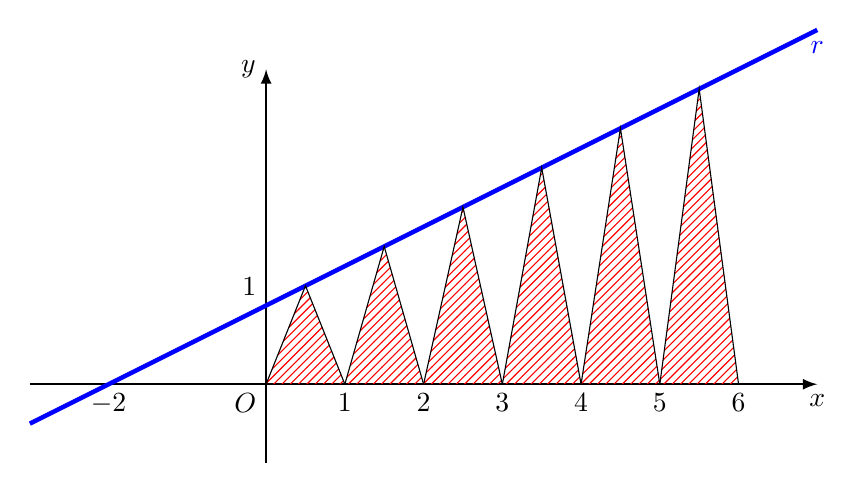
\begin{tikzpicture}
            \draw[->,>=latex,thick] (-3,0) -- (7,0) node[below]{\(x\)};
            \draw[->,>=latex,thick] (0,-1) -- (0,4) node[left]{\(y\)};
            \node at (0,0) [below left]{\(O\)};
            \node at (-2,0) [below]{\(-2\)};
            \node at (0,1) [above left]{\(1\)};
            \tikzmath{
                function calcImage(\x){
                    return 0.5*\x + 1;
                };
            }
            \draw[blue,ultra thick] (-3,-0.5) -- (7,4.5) node[below]{\(r\)};
            \foreach \x in {1,...,6}{
                \draw[pattern color=red, pattern=north east lines] 
                    (\x-1, 0) -- (\x-0.5, {calcImage(\x-0.5)}) -- (\x, 0) 
                    node[below]{\(\x\)}; 
            }
        \end{tikzpicture}
    \end{center}
\end{document}